\documentclass[border=6pt]{standalone}
\usepackage[T1]{fontenc}
\usepackage[utf8]{inputenc}
\usepackage[scaled=0.98]{helvet}
\renewcommand{\familydefault}{\sfdefault}
\usepackage{amsmath}
\usepackage{graphicx}
\graphicspath{{../../../../../../exercises_lecturenotes/lecture_notes/kurs100_lektionsnoter/}}
\usepackage{tikz}
\usepackage{pgfplots}
\pgfplotsset{compat=1.18}
\usetikzlibrary{arrows.meta, decorations.pathreplacing, calc, positioning, fit, backgrounds, shapes.geometric}
\usepgfplotslibrary{groupplots,fillbetween}
\definecolor{scanpink}{HTML}{E5006D}
\definecolor{scanteal}{HTML}{00A6A6}
\definecolor{scannavy}{HTML}{243746}
\definecolor{scanlightgray}{HTML}{F1F2F3}
\begin{document}
  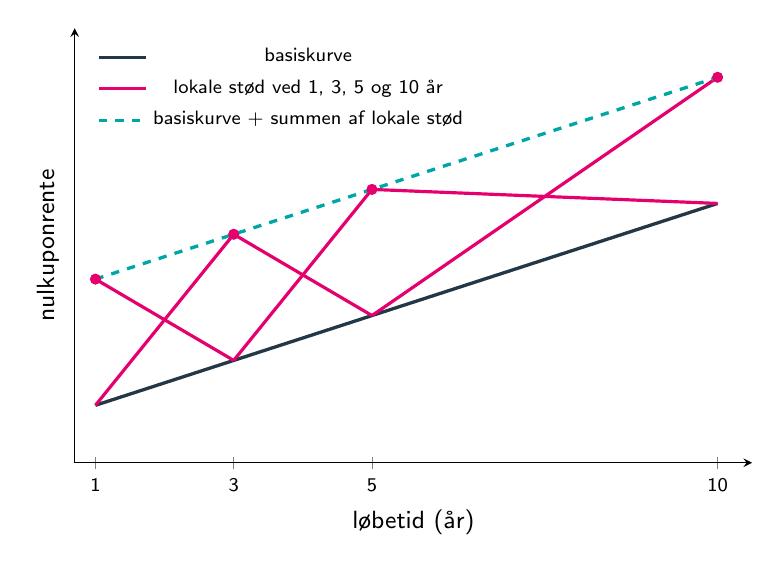
\begin{tikzpicture}

    % Størrelsen på hvert nøglerentestød er kun valgt
    % for at gøre figuren tydelig.
    \pgfmathsetmacro{\shock}{0.90}

    \begin{axis}[
      width=0.84\textwidth,
      height=7.1cm,
      axis lines=left,
      xlabel={løbetid (år)},
      ylabel={nulkuponrente},
      xmin=0.7,
      xmax=10.5,
      ymin=1.1,
      ymax=4.2,
      xtick={1,3,5,10},
      xticklabels={1,3,5,10},
      ytick=\empty,
      legend style={
        draw=none,
        fill=none,
        font=\scriptsize,
        at={(0.02,0.98)},
        anchor=north west,
        row sep=1pt
      },
      tick label style={font=\scriptsize},
      label style={font=\small},
      clip=false
    ]

      % -------------------------------------------------
      % Basiskurve
      % -------------------------------------------------
      \addplot[
        scannavy,
        very thick,
        domain=1:10,
        samples=100
      ]
        {1.35 + 0.16*x};
      \addlegendentry{basiskurve}

      % -------------------------------------------------
      % Lokalt stød til 1-årsrenten
      %
      % Vægten er 1 ved 1 år og falder lineært
      % til 0 ved 3 år.
      % -------------------------------------------------
      \addplot[
        scanpink,
        line width=1.15pt,
        domain=1:3,
        samples=40
      ]
        {1.35 + 0.16*x
         + \shock*(3-x)/2};
      \addlegendentry{lokale stød ved 1, 3, 5 og 10 år}

      % -------------------------------------------------
      % Lokalt stød til 3-årsrenten
      %
      % Vægten stiger fra 0 ved 1 år til 1 ved
      % 3 år og falder derefter til 0 ved 5 år.
      % -------------------------------------------------
      \addplot[
        scanpink,
        line width=1.15pt,
        domain=1:5,
        samples=80,
        forget plot
      ]
        {1.35 + 0.16*x
         + \shock*max(0,min((x-1)/2,(5-x)/2))};

      % -------------------------------------------------
      % Lokalt stød til 5-årsrenten
      %
      % Vægten stiger fra 0 ved 3 år til 1 ved
      % 5 år og falder derefter til 0 ved 10 år.
      % -------------------------------------------------
      \addplot[
        scanpink,
        line width=1.15pt,
        domain=3:10,
        samples=100,
        forget plot
      ]
        {1.35 + 0.16*x
         + \shock*max(0,min((x-3)/2,(10-x)/5))};

      % -------------------------------------------------
      % Lokalt stød til 10-årsrenten
      %
      % Vægten stiger fra 0 ved 5 år til 1 ved
      % 10 år.
      % -------------------------------------------------
      \addplot[
        scanpink,
        line width=1.15pt,
        domain=5:10,
        samples=60,
        forget plot
      ]
        {1.35 + 0.16*x
         + \shock*(x-5)/5};

      % Markering af de fire nøglerenter
      \addplot[
        scanpink,
        only marks,
        mark=*,
        mark size=1.8pt,
        forget plot
      ]
        coordinates {
          (1,2.41)
          (3,2.73)
          (5,3.05)
          (10,3.85)
        };

      % -------------------------------------------------
      % Basiskurven plus summen af alle lokale stød
      %
      % Da de lokale vægte summerer til 1, bliver
      % resultatet et parallelt skift på \shock.
      % -------------------------------------------------
      \addplot[
        scanteal,
        very thick,
        dashed,
        domain=1:10,
        samples=100
      ]
        {1.35 + 0.16*x + \shock};
      \addlegendentry{basiskurve + summen af lokale stød}

    \end{axis}
  \end{tikzpicture}
\end{document}
